%%%%%%%%%%%%%%%%%%%%%%%%%%%%%%%%%%%%%%%%%%%%%%%%%%%%%%%%%%%%%%%%%%%%%%%%%%%%%%%%%%
\begin{frame}[fragile]\frametitle{}
\begin{center}
{\Large Google Cloud Generative AI}
\end{center}
\end{frame}

%%%%%%%%%%%%%%%%%%%%%%%%%%%%%%%%%%%%%%%%%%%%%%%%%%%%%%%%%%%%%%%%%%%%%%%%%%%%%%%%%%
\begin{frame}[fragile]{Concepts}
\begin{itemize}
\item Generative AI trains algorithms to generate new data similar to existing data.
\item Google's generative AI tools use deep learning algorithms and neural networks.
% \item Key concepts include autoencoders, GANs, and VAEs.
\end{itemize}
\end{frame}

%%%%%%%%%%%%%%%%%%%%%%%%%%%%%%%%%%%%%%%%%%%%%%%%%%%%%%%%%%%%%%%%%%%%%%%%%%%%%%%%%%
\begin{frame}[fragile]{Framework}
\begin{itemize}
\item Google provides frameworks like TensorFlow, Keras, and PyTorch for generative AI development.
\item Pre-trained models and APIs like Cloud AutoML and Vertex AI are available.
\end{itemize}
\end{frame}

%%%%%%%%%%%%%%%%%%%%%%%%%%%%%%%%%%%%%%%%%%%%%%%%%%%%%%%%%%%%%%%%%%%%%%%%%%%%%%%%%%
\begin{frame}[fragile]{Vertex AI}

\begin{center}
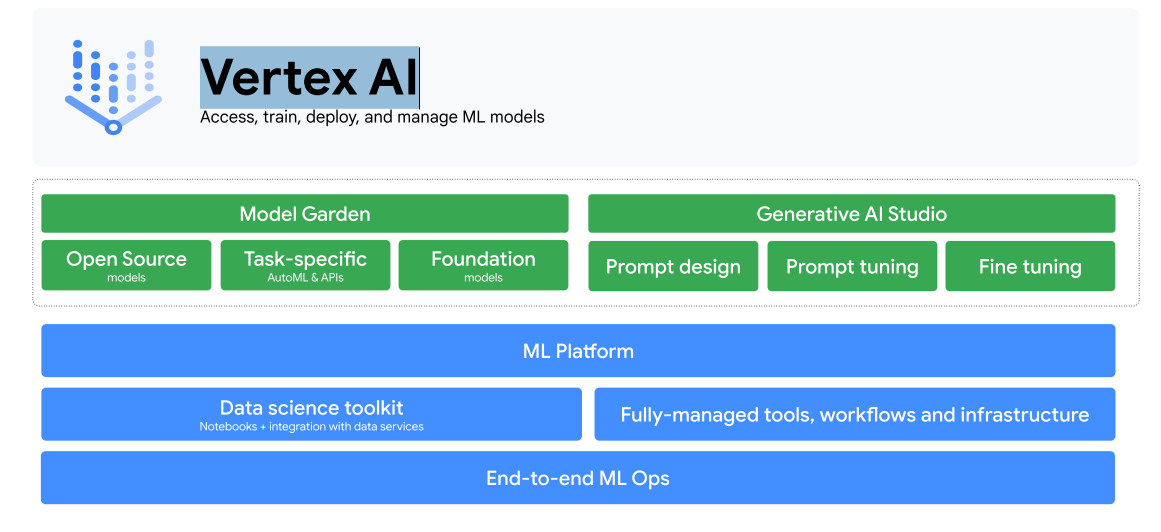
\includegraphics[width=\linewidth,keepaspectratio]{genai9}
\end{center}

{\tiny (Ref: Primer on LLM and Gen AI - Google Cloud)}
  
\end{frame}


%%%%%%%%%%%%%%%%%%%%%%%%%%%%%%%%%%%%%%%%%%%%%%%%%%%%%%%%%%%
\begin{frame}[fragile]\frametitle{Model Garden in Vertex AI}

\begin{center}
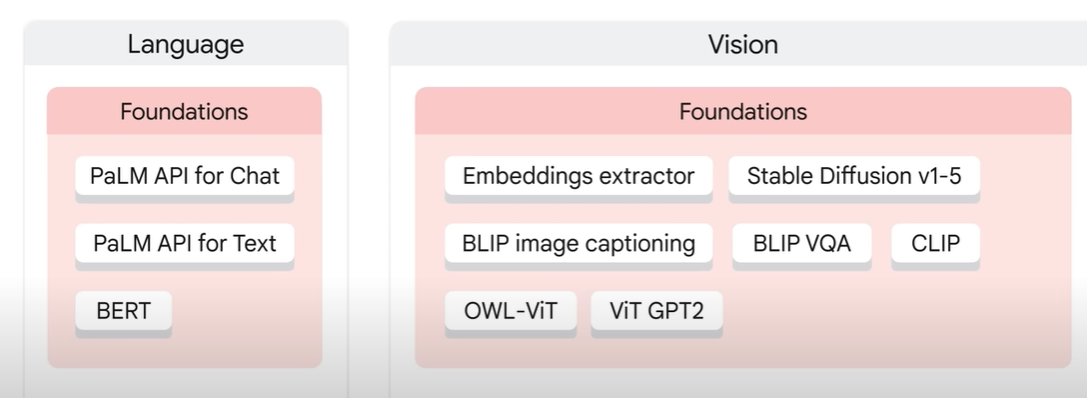
\includegraphics[width=\linewidth,keepaspectratio]{genai22}
\end{center}


{\tiny (Ref: Introduction to Generative AI - Google Cloud Tech)}

\end{frame}

%%%%%%%%%%%%%%%%%%%%%%%%%%%%%%%%%%%%%%%%%%%%%%%%%%%%%%%%%%%
\begin{frame}[fragile]\frametitle{Gen AI Studio}

\begin{center}
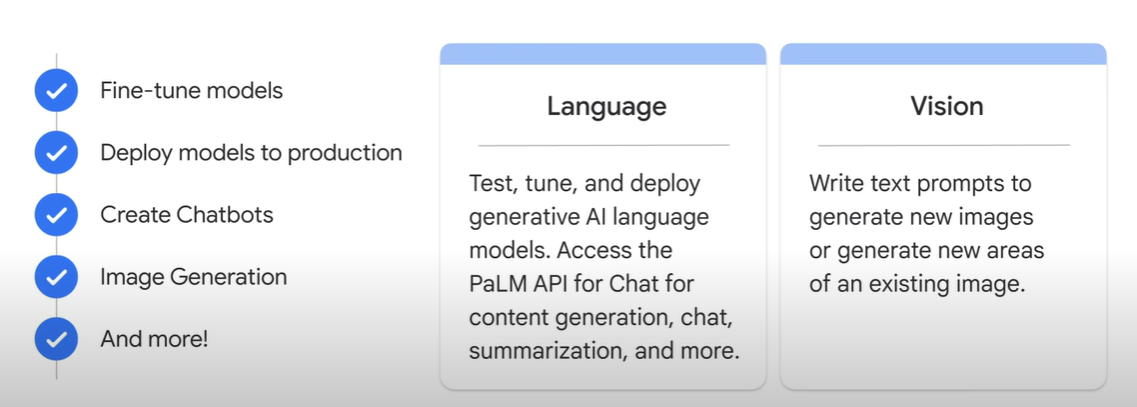
\includegraphics[width=\linewidth,keepaspectratio]{genai23}
\end{center}


{\tiny (Ref: Introduction to Generative AI - Google Cloud Tech)}

\end{frame}


%%%%%%%%%%%%%%%%%%%%%%%%%%%%%%%%%%%%%%%%%%%%%%%%%%%%%%%%%%%
\begin{frame}[fragile]\frametitle{Gen AI App Builder}

Drag and drop Interface, easy to build apps. You can create digial assitants, custom search engine, etc.

\begin{center}
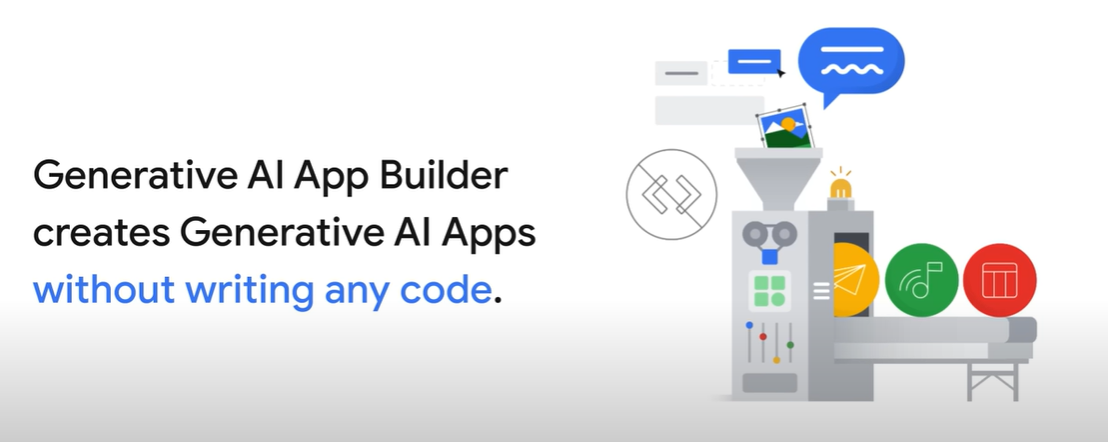
\includegraphics[width=\linewidth,keepaspectratio]{genai24}
\end{center}


{\tiny (Ref: Introduction to Generative AI - Google Cloud Tech)}

\end{frame}

%%%%%%%%%%%%%%%%%%%%%%%%%%%%%%%%%%%%%%%%%%%%%%%%%%%%%%%%%%%
\begin{frame}[fragile]\frametitle{Gen AI Development Cycle}

\begin{center}
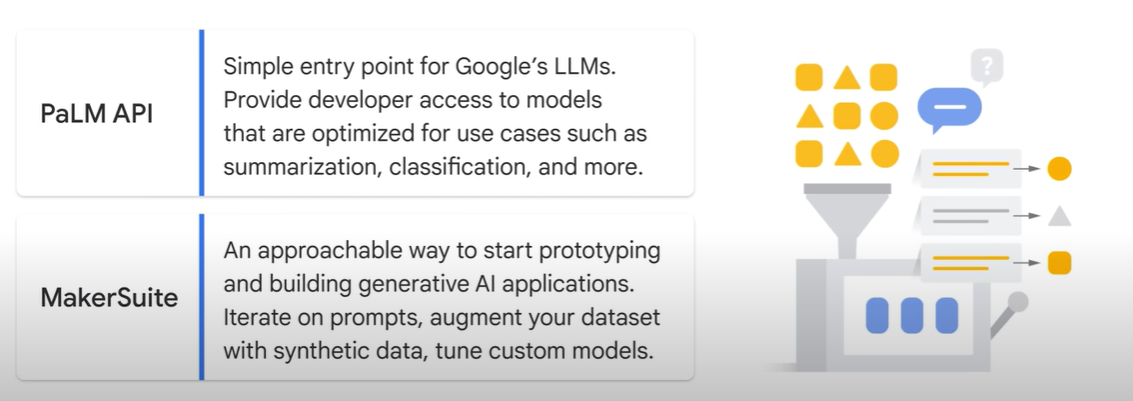
\includegraphics[width=\linewidth,keepaspectratio]{genai25}
\end{center}


{\tiny (Ref: Introduction to Generative AI - Google Cloud Tech)}

\end{frame}


%%%%%%%%%%%%%%%%%%%%%%%%%%%%%%%%%%%%%%%%%%%%%%%%%%%%%%%%%%%%%%%%%%%%%%%%%%%%%%%%%%
\begin{frame}[fragile]{Applications}
\begin{itemize}
\item Generative AI applies to image/video generation, natural language processing, and music composition.
\item Google's tools are used in healthcare, finance, entertainment, and more.
\item Applications include Gmail, Docs, Slides, Sheets, and others.
\end{itemize}
\end{frame}

%%%%%%%%%%%%%%%%%%%%%%%%%%%%%%%%%%%%%%%%%%%%%%%%%%%%%%%%%%%
\begin{frame}[fragile]\frametitle{Applications to Creative Field}

\begin{center}
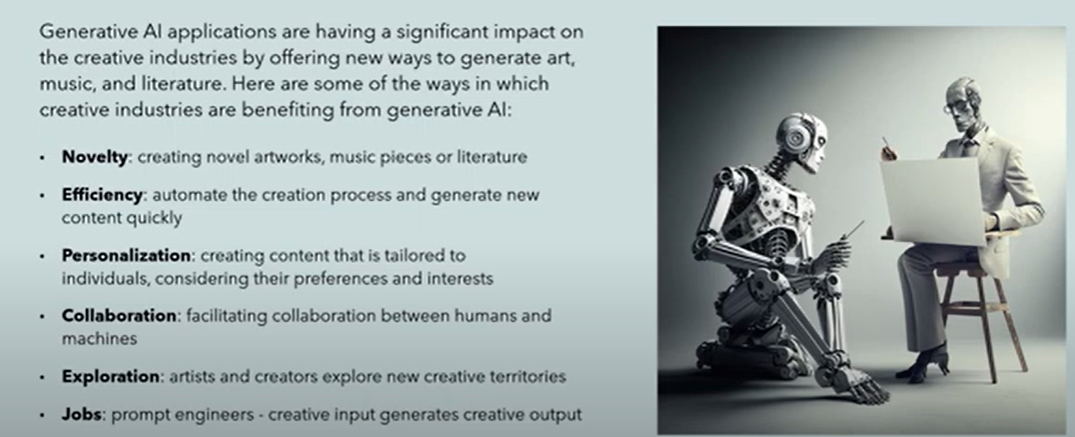
\includegraphics[width=\linewidth,keepaspectratio]{genai27}
\end{center}


{\tiny (Ref: Generative AI Presentation  - Laura Worden)}

\end{frame}

%%%%%%%%%%%%%%%%%%%%%%%%%%%%%%%%%%%%%%%%%%%%%%%%%%%%%%%%%%%
\begin{frame}[fragile]\frametitle{Applications to Art}

\begin{center}
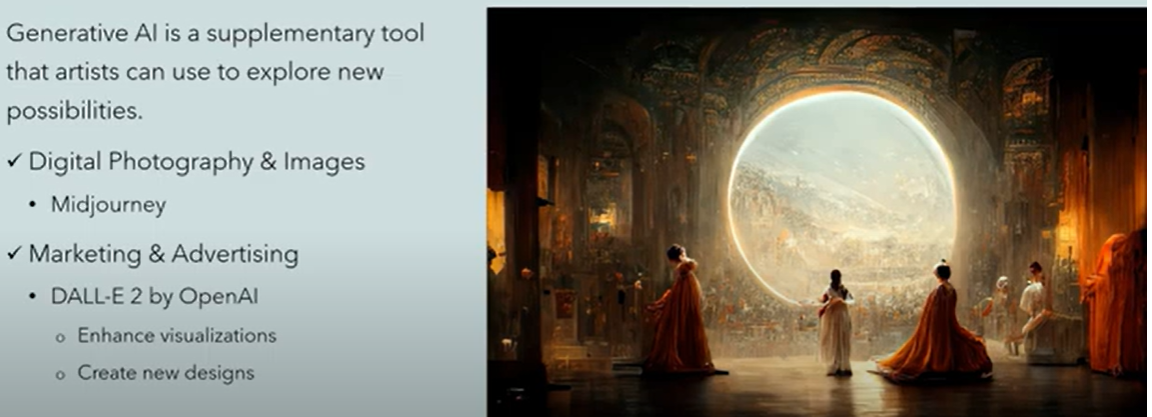
\includegraphics[width=\linewidth,keepaspectratio]{genai28}
\end{center}


{\tiny (Ref: Generative AI Presentation  - Laura Worden)}

\end{frame}

%%%%%%%%%%%%%%%%%%%%%%%%%%%%%%%%%%%%%%%%%%%%%%%%%%%%%%%%%%%
\begin{frame}[fragile]\frametitle{Applications to Music}

\begin{center}
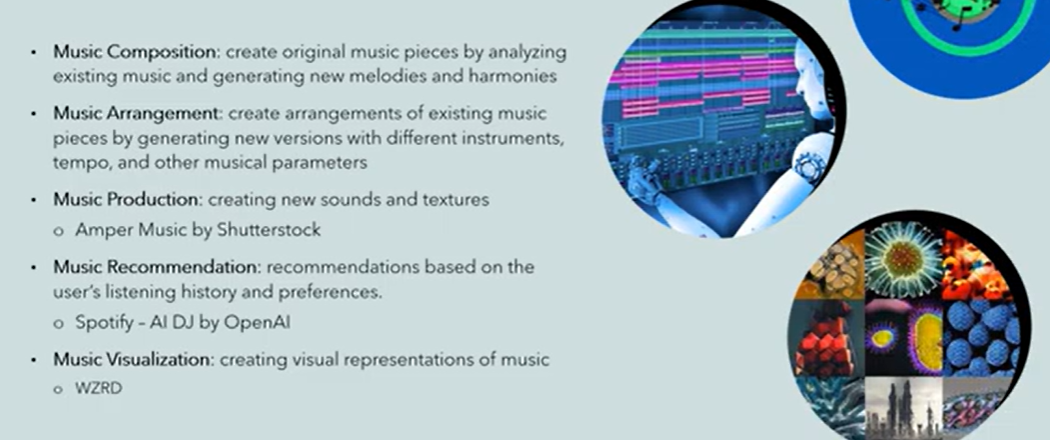
\includegraphics[width=\linewidth,keepaspectratio]{genai29}
\end{center}


{\tiny (Ref: Generative AI Presentation  - Laura Worden)}

\end{frame}

%%%%%%%%%%%%%%%%%%%%%%%%%%%%%%%%%%%%%%%%%%%%%%%%%%%%%%%%%%%
\begin{frame}[fragile]\frametitle{Applications to Literature}

\begin{center}
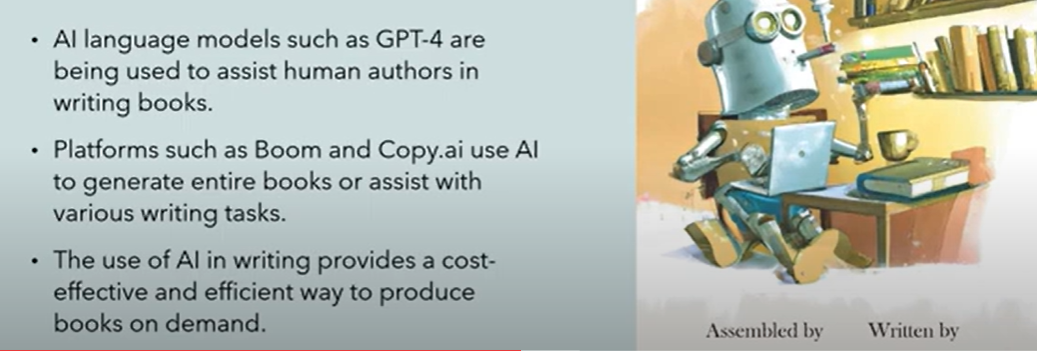
\includegraphics[width=\linewidth,keepaspectratio]{genai30}
\end{center}


{\tiny (Ref: Generative AI Presentation  - Laura Worden)}

\end{frame}

%%%%%%%%%%%%%%%%%%%%%%%%%%%%%%%%%%%%%%%%%%%%%%%%%%%%%%%%%%%
\begin{frame}[fragile]\frametitle{Applications to Healthcare}

\begin{center}
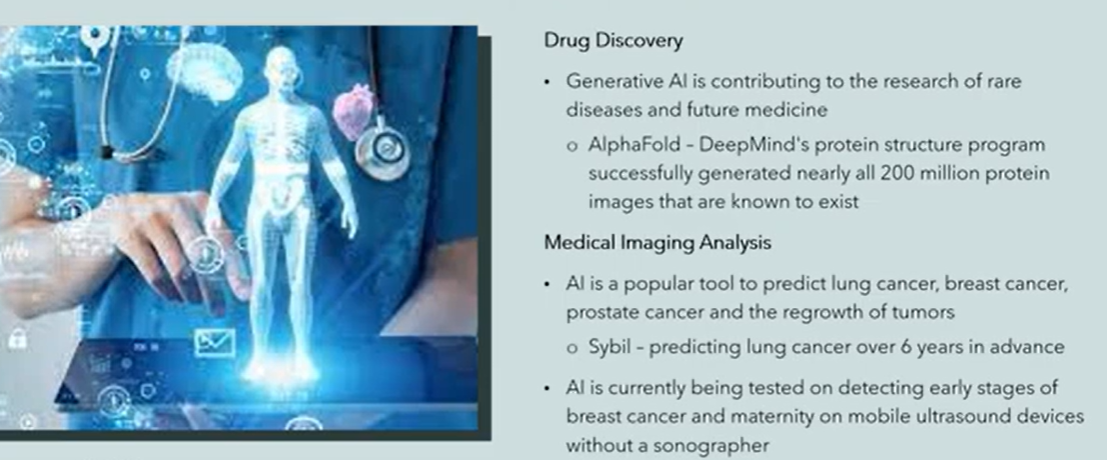
\includegraphics[width=\linewidth,keepaspectratio]{genai31}
\end{center}


{\tiny (Ref: Generative AI Presentation  - Laura Worden)}

\end{frame}

%%%%%%%%%%%%%%%%%%%%%%%%%%%%%%%%%%%%%%%%%%%%%%%%%%%%%%%%%%%
\begin{frame}[fragile]\frametitle{Applications to Gaming}

\begin{center}
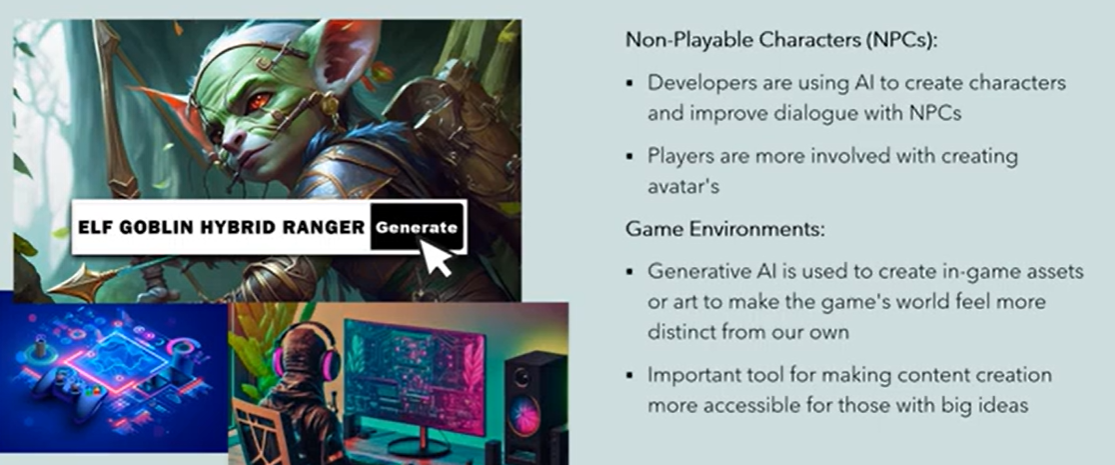
\includegraphics[width=\linewidth,keepaspectratio]{genai32}
\end{center}


{\tiny (Ref: Generative AI Presentation  - Laura Worden)}

\end{frame}



%%%%%%%%%%%%%%%%%%%%%%%%%%%%%%%%%%%%%%%%%%%%%%%%%%%%%%%%%%%
\begin{frame}[fragile]\frametitle{Advantages of Gen AI}

\begin{center}
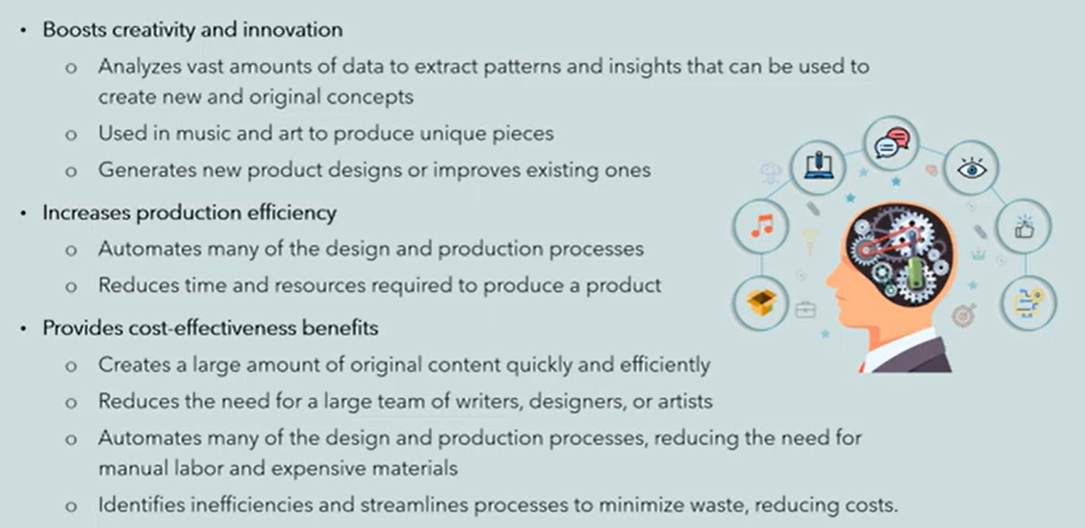
\includegraphics[width=\linewidth,keepaspectratio]{genai26}
\end{center}


{\tiny (Ref: Generative AI Presentation  - Laura Worden)}

\end{frame}

%%%%%%%%%%%%%%%%%%%%%%%%%%%%%%%%%%%%%%%%%%%%%%%%%%%%%%%%%%%
\begin{frame}[fragile]\frametitle{Risks of Gen AI}
Ethical concerns

\begin{center}
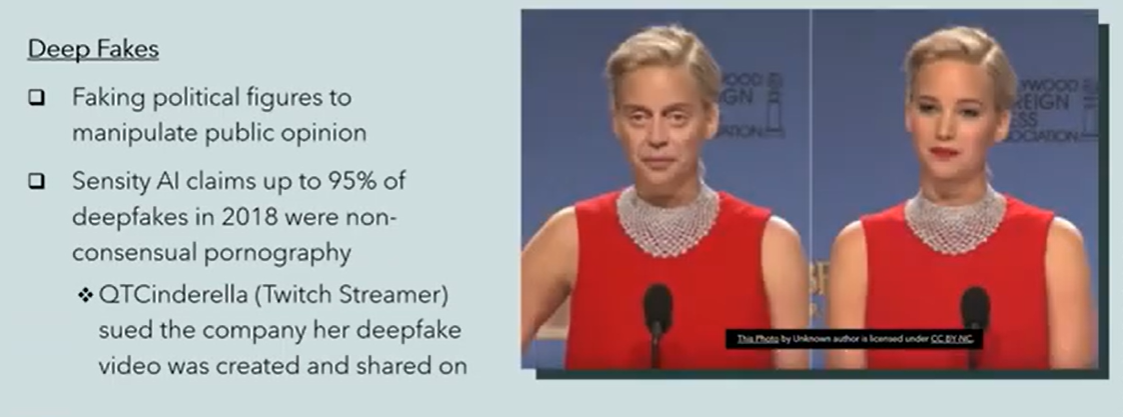
\includegraphics[width=\linewidth,keepaspectratio]{genai33}
\end{center}


{\tiny (Ref: Generative AI Presentation  - Laura Worden)}

\end{frame}

%%%%%%%%%%%%%%%%%%%%%%%%%%%%%%%%%%%%%%%%%%%%%%%%%%%%%%%%%%%
\begin{frame}[fragile]\frametitle{Risks of Gen AI}
Jobs

\begin{center}
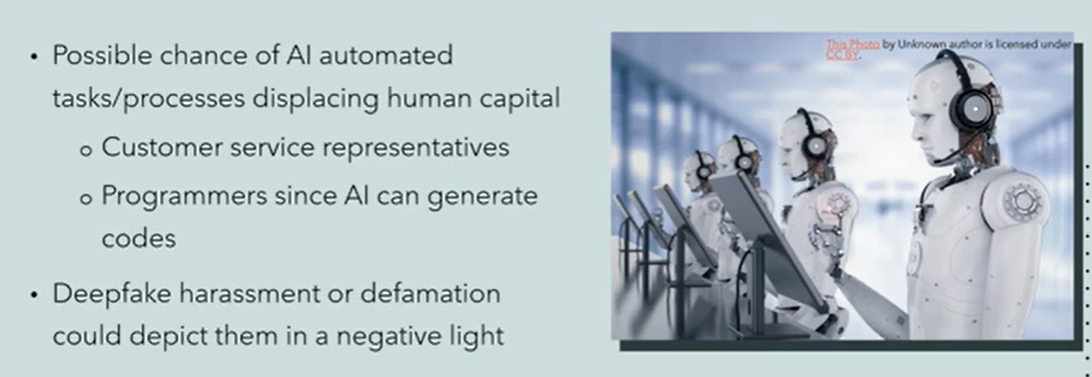
\includegraphics[width=\linewidth,keepaspectratio]{genai34}
\end{center}


{\tiny (Ref: Generative AI Presentation  - Laura Worden)}

\end{frame}

%%%%%%%%%%%%%%%%%%%%%%%%%%%%%%%%%%%%%%%%%%%%%%%%%%%%%%%%%%%
\begin{frame}[fragile]\frametitle{Risks of Gen AI}

Privacy

\begin{center}
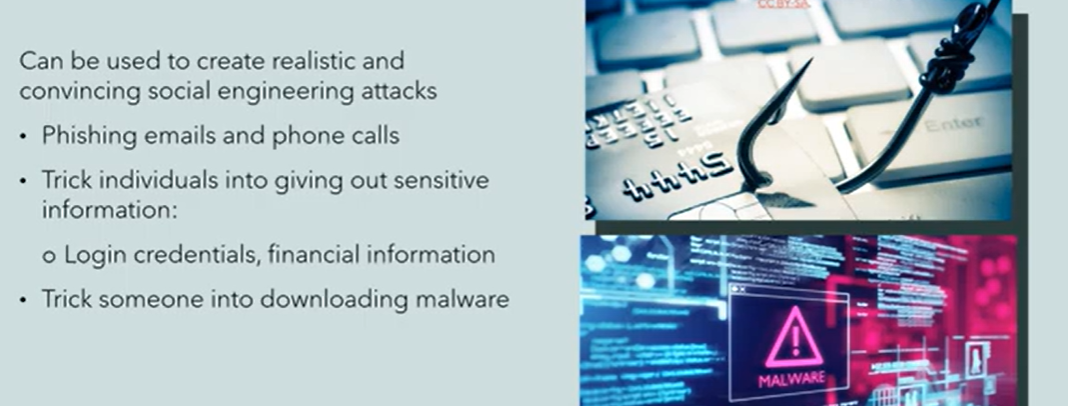
\includegraphics[width=\linewidth,keepaspectratio]{genai35}
\end{center}


{\tiny (Ref: Generative AI Presentation  - Laura Worden)}

\end{frame}

%%%%%%%%%%%%%%%%%%%%%%%%%%%%%%%%%%%%%%%%%%%%%%%%%%%%%%%%%%%
\begin{frame}[fragile]\frametitle{Mitigation Risks of Gen AI}

Arguments and Rebuttal

\begin{center}
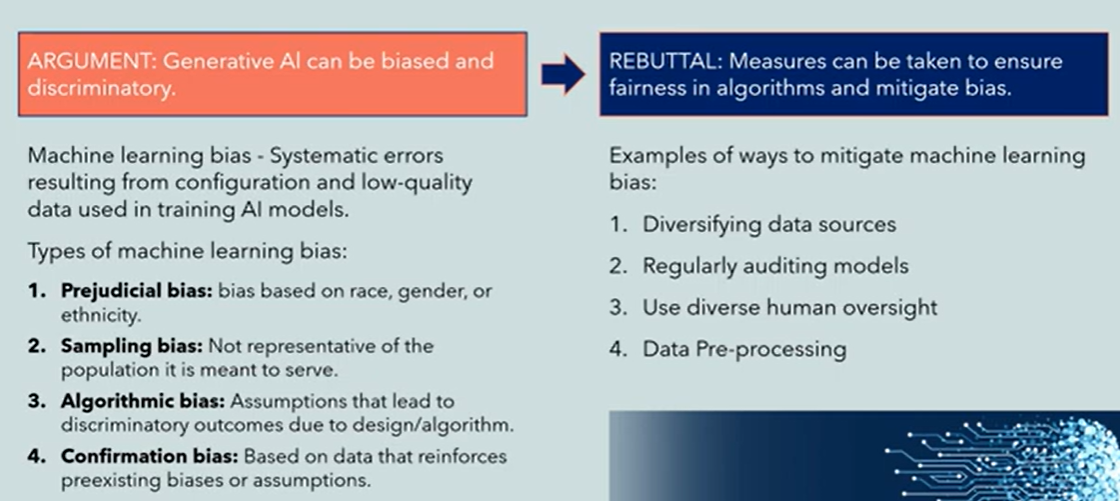
\includegraphics[width=\linewidth,keepaspectratio]{genai36}
\end{center}


{\tiny (Ref: Generative AI Presentation  - Laura Worden)}

\end{frame}

%%%%%%%%%%%%%%%%%%%%%%%%%%%%%%%%%%%%%%%%%%%%%%%%%%%%%%%%%%%
\begin{frame}[fragile]\frametitle{Mitigation Risks of Gen AI}

Arguments and Rebuttal

\begin{center}
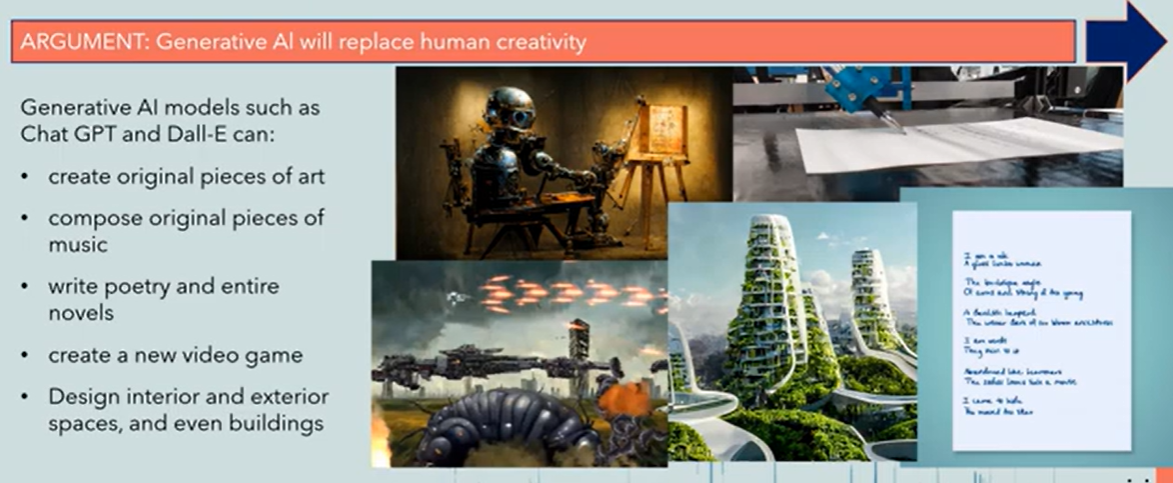
\includegraphics[width=\linewidth,keepaspectratio]{genai37}
\end{center}


{\tiny (Ref: Generative AI Presentation  - Laura Worden)}

\end{frame}



%%%%%%%%%%%%%%%%%%%%%%%%%%%%%%%%%%%%%%%%%%%%%%%%%%%%%%%%%%%%%%%%%%%%%%%%%%%%%%%%%%
\begin{frame}[fragile]{Conclusion}
\begin{itemize}
\item Google's generative AI is a powerful technology with potential industry revolution.
\item Google leads with frameworks, tools, and pre-trained models.
\item Expect more innovative applications as the technology advances.
\end{itemize}
\end{frame}

%%%%%%%%%%%%%%%%%%%%%%%%%%%%%%%%%%%%%%%%%%%%%%%%%%%%%%%%%%%%%%%%%%%%%%%%%%%%%%%%%%
\begin{frame}[fragile]{References}

\begin{center}
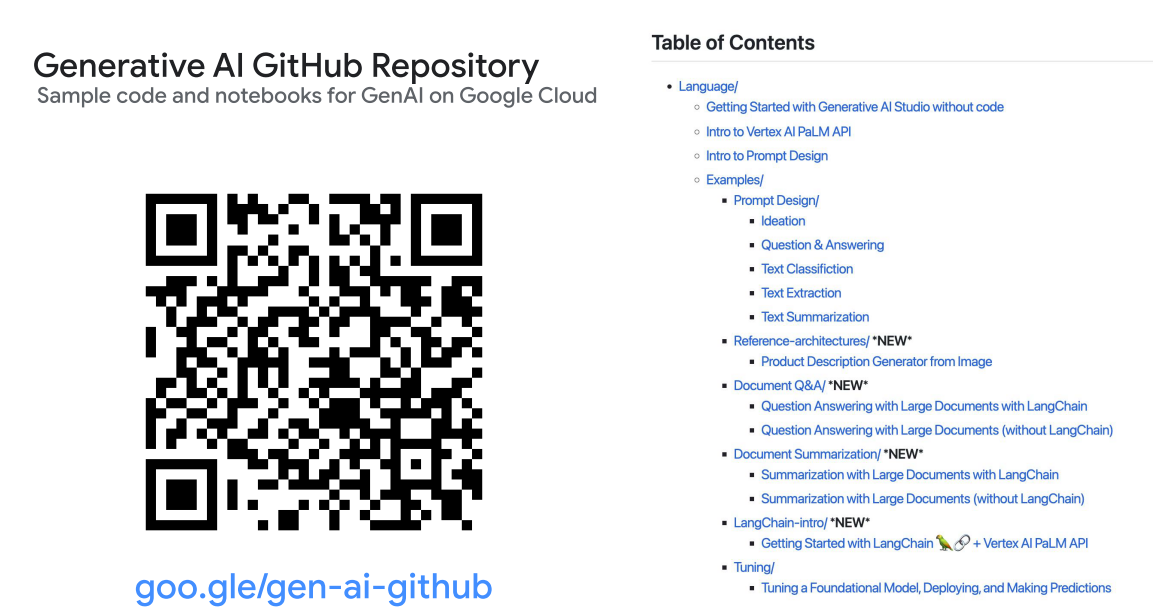
\includegraphics[width=\linewidth,keepaspectratio]{genai10}
\end{center}

{\tiny (Ref: Primer on LLM and Gen AI - Google Cloud)}
  
\end{frame}